\documentclass[main.tex]{subfiles}

\begin{document}

% \textcolor{red}{Вводная лекция}

\section{Лекция 08.04.2021 (Валов А.В.)}

\subsection{Модель Planar3D ILSA: дискретизация, поиск фронта, алгоритм}

Продолжаем разрабатывать численный алгоритм для модели Planar3D ILSA.

\subsubsection{Дискретизация уравнений. Продолжение}

В прошлый раз остановились на дискретизации уравнения Рейнольдса.
А именно проинтегрировали его по одному шагу по времени и, воспользовавшись формулой Ньютона-Лейбница и формулой правых прямоугольников, получили:
\beq
w(t)-w(t-\Delta t)-\Delta t\left[\text{div}{\left(\frac{w^3}{\mu'}\nabla p\right)}\right]_t=\int\limits_{t-\Delta t}^{t}{\varphi(\tau)d\tau}
\eeq


\textbf{Дискретизация уравнения Рейнольдса. Продолжение}

Далее проинтегрируем полученное уравнение по элементам.
Запишем:
\beq\label{RaynoldsIntegrateOnElements1}
\int\limits_{A_{i,j}}{\left(w(t)-w(t-\Delta t)\right)dA}-\Delta t\left[\,\,\int\limits_{A_{i,j}}{\text{div}{\left(\frac{w^3}{\mu'}\nabla p\right)}dA}\right]_t=\int\limits_{t-\Delta t}^{t}{\psi(\tau)d\tau},
\eeq
где
\beq
\psi(t)=\int\limits_{A_{i,j}}{\left(Q_0(t)\delta(x-x_0,y-y_0)-\frac{C'}{\sqrt{t-t_0(x,y)}}\right)dA}
\eeq

Вспомним теорему Гаусса-Остроградского
$$\int\limits_{V}\text{div}\vec{f}\,dV=\int\limits_{\partial V}\vec{f}\cdot\vec{n}\,ds$$
и перепишем уравнение \eqref{RaynoldsIntegrateOnElements1} в следующем виде:
\beq\label{RaynoldsIntegrateOnElements2}
\int\limits_{A_{i,j}}{\left(w(t)-w(t-\Delta t)\right)dA}-\Delta t\left[\,\,\int\limits_{C_{i,j}}{\frac{w^3}{\mu'}\frac{\partial p}{\partial\vec{n}}dC}\right]_t=\int\limits_{t-\Delta t}^{t}{\psi(\tau)d\tau}
\eeq
Здесь дополнительно воспользовались равенством: $\nabla p\cdot\vec{n}=\dfrac{\partial p}{\partial\vec{n}}$.

С полученным уравнением \eqref{RaynoldsIntegrateOnElements2} уже можно работать.

Напомню, что раскрытие трещины $w(x,y,t)$ аппроксимируем кусочно-постоянно:
\beq
w(x,y,t)=\sum_{m,n}w_{m,n}(t)H_{m,n}(x,y),
\eeq
где
\beq
H_{i,j}(x,y)=
\begin{cases}
1,\,\,\,(x,y)\in A_{i,j}\\
0,\,\,\,(x,y)\notin A_{i,j}	
\end{cases}
\eeq

После подстановки кусочно-постоянного раскрытия $w$ слагаемые в уравнении \eqref{RaynoldsIntegrateOnElements2} перепишутся в следующем виде:
\beq
\int\limits_{A_{i,j}}{\left(w(t)-w(t-\Delta t)\right)dA}=\left(w_{i,j}(t)-w_{i,j}(t-\Delta t)\right)\Delta x\Delta y
\eeq
(т.к. раскрытие кусочно-постоянно);

\begin{multline}
\int\limits_{t-\Delta t}^{t}{\psi(\tau)d\tau}=\int\limits_{A_{i,j}}\,{\int\limits_{t-\Delta t}^{t}{\left(Q_0(t)\delta(x-x_0,y-y_0)-\frac{C'}{\sqrt{t-t_0(x,y)}}\right)d\tau}\,dA}\approx\\
\approx \Delta x\Delta y\Delta t\left[Q_{i,j}\right]_t-2C'\Delta x\Delta y\left(\sqrt{t-t_{0_{i,j}}}-\sqrt{t-\Delta t-t_{0_{i,j}}}\right)
\end{multline}
(здесь воспользовались формулой средних прямоугольников при интегрировании по ячейке и формулой правых прямоугольников при интегрировании по временному шагу; полученная формула верна только для внутренних элементов, так как при использовании формулы средних прямоугольников берём значение функции только в центре элемента; для концевых элементов выведем формулу позже);

\begin{multline}
\int\limits_{C_{i,j}}{\frac{w^3}{\mu'}\frac{\partial p}{\partial\vec{n}}dC}=
\int\limits_{C_{i,j}^{\text{ right}}}{\frac{w^3}{\mu'}\frac{\partial p}{\partial\vec{n}}dC}+
\int\limits_{C_{i,j}^{\text{ left}}}{\frac{w^3}{\mu'}\frac{\partial p}{\partial\vec{n}}dC}+
\int\limits_{C_{i,j}^{\text{ top}}}{\frac{w^3}{\mu'}\frac{\partial p}{\partial\vec{n}}dC}+
\int\limits_{C_{i,j}^{\text{ bot}}}{\frac{w^3}{\mu'}\frac{\partial p}{\partial\vec{n}}dC}\approx\\\\\approx
\underbrace{\frac{w_{i+1,j}^3+w_{i,j}^3}{2\mu'}}_{\text{обозначим за }M_{i+\frac{1}{2},j}}\frac{p_{i+1,j}-p_{i,j}}{\Delta x}\Delta y-
\underbrace{\frac{w_{i,j}^3+w_{i-1,j}^3}{2\mu'}}_{\text{обозначим за }M_{i-\frac{1}{2},j}}\frac{p_{i,j}-p_{i-1,j}}{\Delta x}\Delta y\,+\\\\
+\underbrace{\frac{w_{i,j+1}^3+w_{i,j}^3}{2\mu'}}_{\text{обозначим за }M_{i,j+\frac{1}{2}}}\frac{p_{i,j+1}-p_{i,j}}{\Delta y}\Delta x-
\underbrace{\frac{w_{i,j}^3+w_{i,j-1}^3}{2\mu'}}_{\text{обозначим за }M_{i,j-\frac{1}{2}}}\frac{p_{i,j}-p_{i,j-1}}{\Delta y}\Delta x=\\\\
=\left(M_{i+\frac{1}{2},j}\frac{p_{i+1,j}-p_{i,j}}{\Delta x}-
M_{i-\frac{1}{2},j}\frac{p_{i,j}-p_{i-1,j}}{\Delta x}\right)\Delta y\,+\\\\
+\left(M_{i,j+\frac{1}{2}}\frac{p_{i,j+1}-p_{i,j}}{\Delta y}-
M_{i,j-\frac{1}{2}}\frac{p_{i,j}-p_{i,j-1}}{\Delta y}\right)\Delta x
\end{multline}
(идея здесь такая: разбиваем интеграл по границе на сумму интегралов по кусочкам границы; аппроксимируем подынтегральную функцию на каждом кусочке и считаем интеграл).


Таким образом, уравнение \eqref{RaynoldsIntegrateOnElements2} перепишется в следующем виде:
\beq
\left(w_{i,j}(t)-w_{i,j}(t-\Delta t)\right)\Delta x\Delta y=\Delta x\Delta y\Delta t\left[Ap\right]_{i,j}+\Delta x\Delta y\Delta t\,Q_{i,j}-\Delta x\Delta y\Delta L_{i,j},
\eeq
где
\begin{multline}
[Ap]_{i,j}=\frac{1}{\Delta x}
\left[M_{i+\frac{1}{2},j}\frac{p_{i+1,j}-p_{i,j}}{\Delta x}-M_{i-\frac{1}{2},j}\frac{p_{i,j}-p_{i-1,j}}{\Delta x}\right]+\\\\
+\frac{1}{\Delta y}
\left[M_{i,j+\frac{1}{2}}\frac{p_{i,j+1}-p_{i,j}}{\Delta y}-M_{i,j-\frac{1}{2}}\frac{p_{i,j}-p_{i,j-1}}{\Delta y}\right]
\end{multline}

Вспомним, что у нас есть дополнительное граничное условие нулевого потока на границе трещины:
\beq
\vec{q}\cdot\vec{n}\mathop{=}_{s\to 0}0
\eeq

Чтобы удовлетворить этому условию нулевого потока на границе, необходимо занулить потоки через внешние границы концевых элементов.
\\

Лирическое отступление.
В интернете есть \href{https://www.youtube.com/watch?v=PXfy5f9kWh4}{оригинальная лекция} Энтони Пирса (Anthony Peirce).
Можете ради интереса посмотреть её.
Там есть некоторые нюансы, которые мы сегодня опустили: например, метод микроскопа.
Изначально модель была придумана не с универсальной асимптотикой.
Если проследить эволюцию статей, то можно посмотреть, как развивалась мысль.
\\

Итак, на текущий момент мы разобрались с уравнением упругости (его мы просто взяли и проинтегрировали), разобрались с уравнением Рейнольдса (выписали схему конечных объёмов).
Теперь необходимо разобраться, зачем мы делили элементы на внутренние, опорные и концевые.


\subsubsection{Зачем вводили классификацию элементов?}

У нас есть граничное условие: $\displaystyle{}w\mathop{\sim}_{s\to 0}w_a(s)$
Мы будем его использовать, чтобы определять положение фронта и раскрытие в концевых элементах.

\begin{center}
\includegraphics[width=.6\textwidth, page=6]{Valov_slides.pdf}
\end{center}

\begin{center}
\includegraphics[width=.6\textwidth, page=7]{Valov_slides.pdf}
\end{center}






\end{document}